\chapter{A Dual Chamber Pacemaker Specification}

\begin{itemize}
	\item What are the basic functions?
   \item What happens if new functionality are applied to the basic model?
\end{itemize}
The software component of medical devices are becoming more and more complex. Problems may arise when adding new functionality to already verified software. In this chapter we demonstrate the basic specification of a dual chamber pacemaker, as well as a mode-switch function on top of the basic functions. The specifications are based on the algorithm description in \cite{compass}.
\begin{figure}[!t]
\center
%\vspace{-10pt}
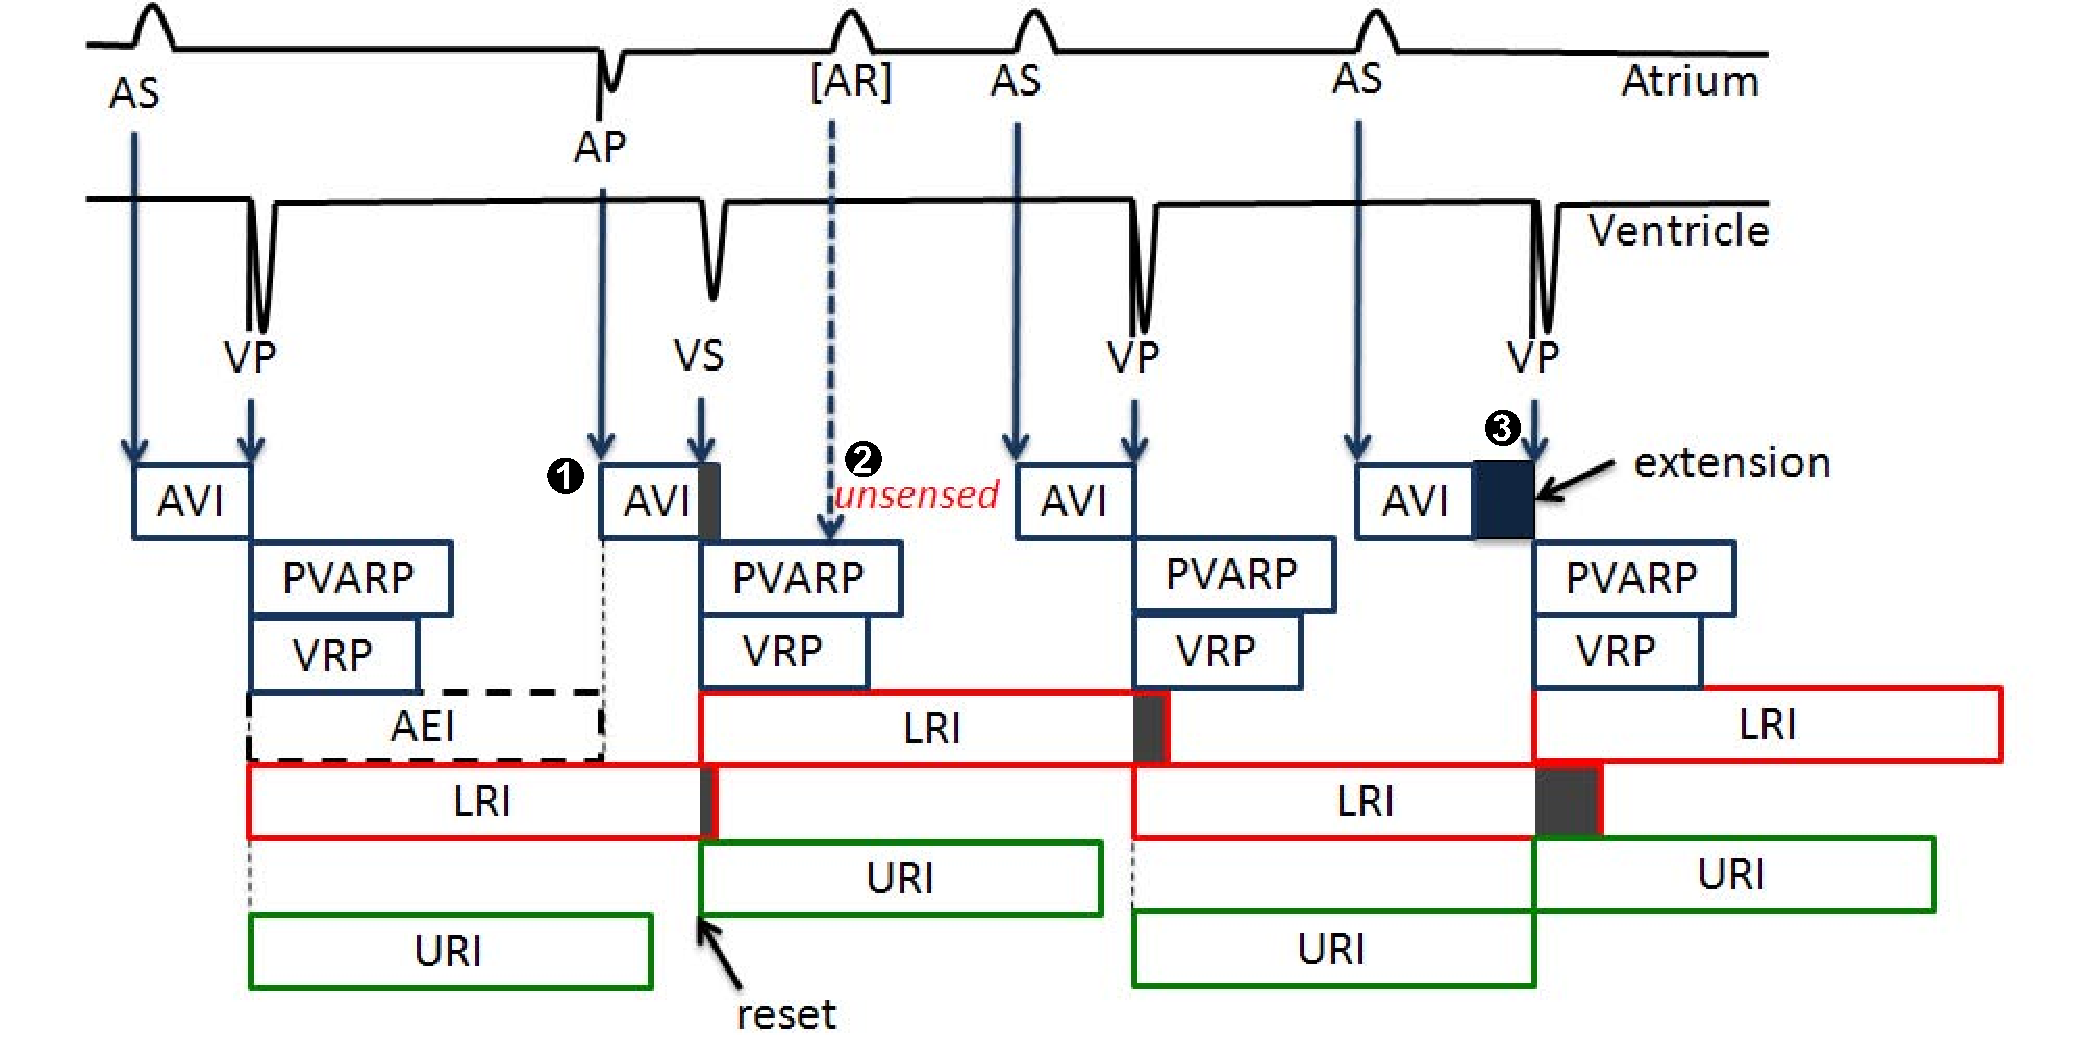
\includegraphics[width=0.7\textwidth]{figs/PM_timers.pdf}
%\vspace{-10pt}
\caption{Basic 5 timing cycles for a dual chamber pacemaker}
\label{fig:PMtimers}
%\vspace{-10pt}t

\end{figure} 
\section{Basic Specifications of a DDD Pacemaker}

The DDD pacemaker has 5 basic timing cycles triggered by external and internal events, as shown in \figref{PMtimers}. We decomposed our pacemaker model into 5 components which correspond to the 5 timers. $P=LRI\| AVI\| URI\| PVARP\| VRP$. These components synchronize with each other using broadcast channels and shared variables (as shown in \figref{PMdesign}). 

\subsection{Lower Rate Interval (LRI)}
%\vspace{-5pt}
The Lower Rate Interval (LRI) component is shown in \figref{PMdesign}(a). This component defines the longest interval allowed between two ventricular events, thus keeping the heart rate above a minimum value. In DDD mode, the LRI interval is divided into a V-A interval (TLRI-TAVI) and a A-V interval (TAVI). The LRI component maintains a maximum V-A delay while the AVI component maintains a maximum A-V delay so together they maintain the maximum V-V delay. In the LRI component, the clock is reset when a ventricular event \textsf{(VS, VP)} is received. If no atrial event has been sensed \textsf{(AS)}, the component will deliver atrial pacing \textsf{(AP)} after TLRI-TAVI. 

%\vspace{-5pt}
\subsection{Atrio-Ventricular Interval (AVI) and Upper Rate Interval (URI)}
%\vspace{-5pt}
The function of the AVI component defines the longest interval between an atrial event and a ventricular event. If there is no ventricular event \textsf{(VS)}  within TAVI after an atrial event \textsf{(AS, AP)}, and the time since the last ventricular event \textsf{(VS, VP)} is longer than TURI, the component will deliver ventricular pacing \textsf{(VP)}. The URI limits the ventricular pacing rate by enforcing a lower bound on the times between consecutive ventricle events. The UPPAAL design of AVI and URI component is shown in \figref{PMdesign}(b) and (c).%The UPPAAL design of AVI component is shown in 

%\vspace{-10pt}
\subsection{Post Ventricular Atrial Refractory Period (PVARP) and Post Ventricular Atrial Blanking (PVAB)}
%\vspace{-5pt}
Ventricular events, especially Ventricular Pace (VP) are sometimes so strong that the atrial lead can sense the activation as well. This signal may be falsely recognized as an atrial event and disrupt normal pacemaker function. This scenario is called crosstalk and was discussed in our previous work \cite{vhm_embc11}. In order to prevent this undesired behavior, and filter potential noises, there is a blanking period (PVAB) followed by a refractory period (PVARP) for the atrial events after each ventricular event \textsf{(VS, VP)}. Atrial events during PVAB are ignored and atrial events during PVARP trigger \textsf{AR!} events which can be used in some advanced diagnostic algorithms. The UPPAAL design of PVARP component is shown in \figref{PMdesign}(d).

%\vspace{-10pt}
\subsection{Ventricular Refractory Period (VRP)}
%\vspace{-5pt}
Correspondingly, the VRP follows each ventricular event \textsf{(VP, VS)} to filter noise and early events in the ventricular channel which could otherwise cause undesired pacemaker behavior. \figref{PMdesign}(e) shows the UPPAAL design of VRP component.

\begin{figure}[!t]
\center
%\vspace{-10pt}
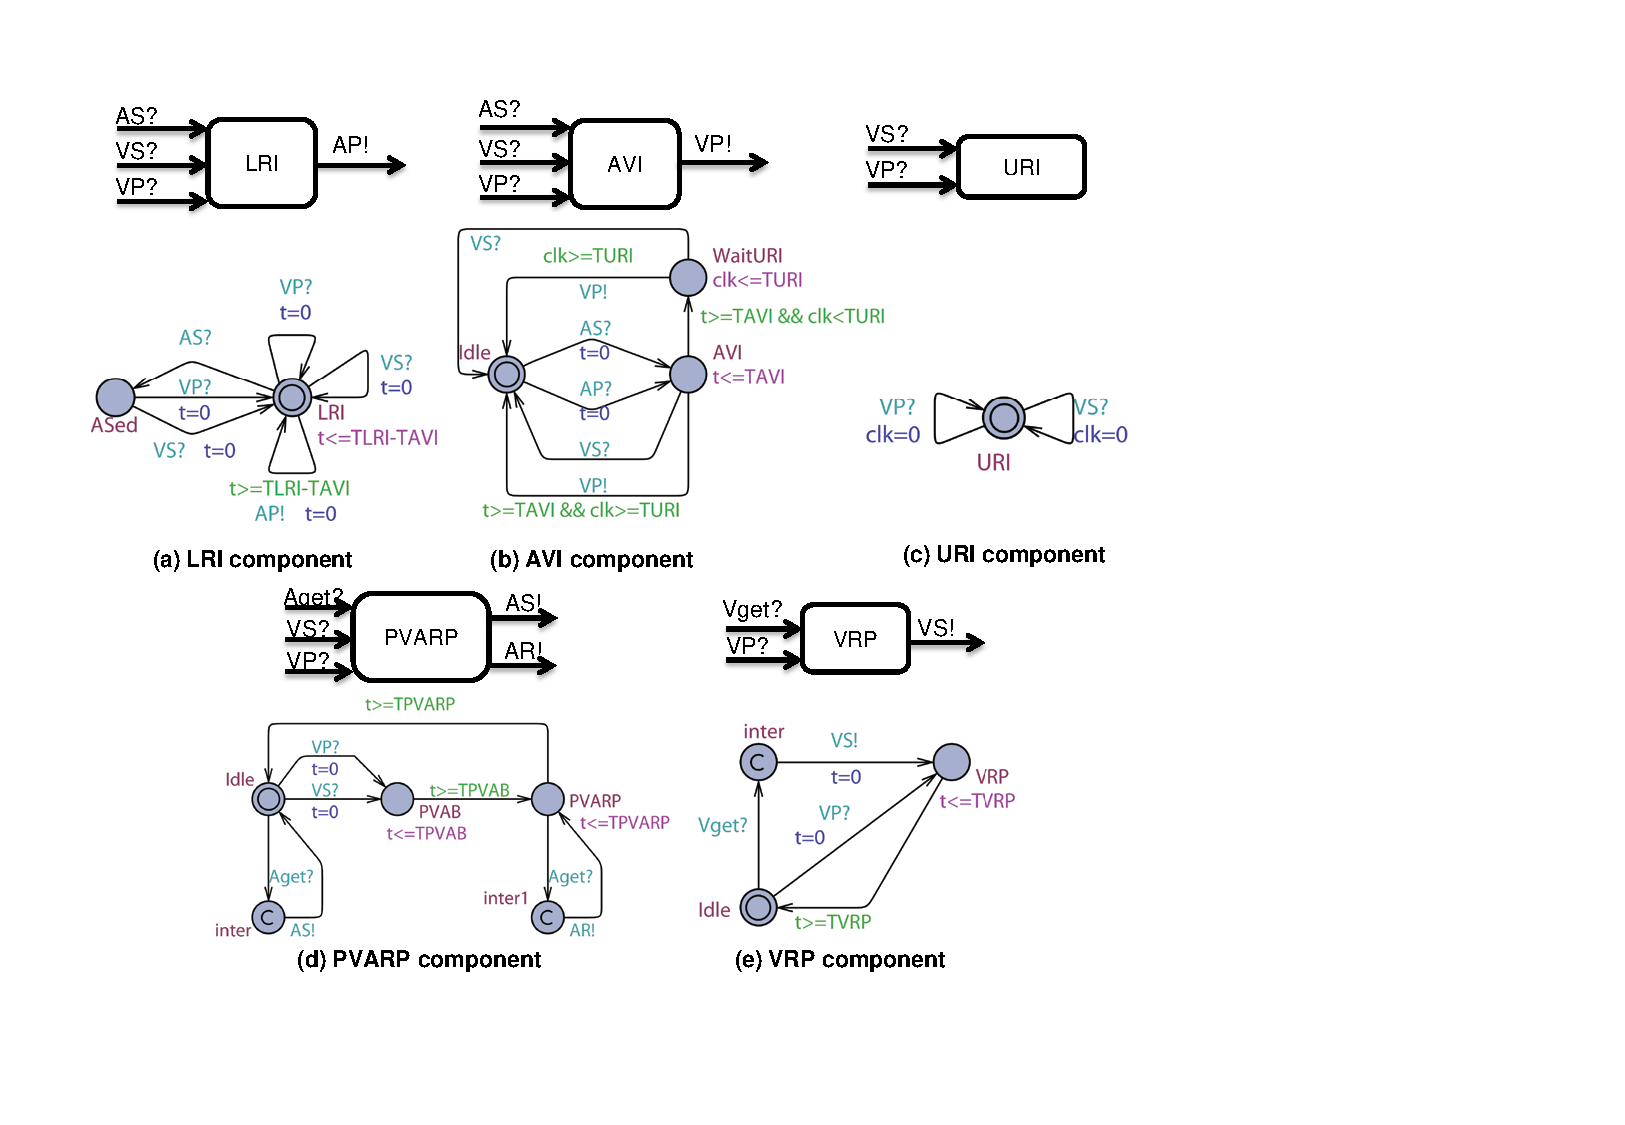
\includegraphics[width=0.9\textwidth]{figs/pacemaker.pdf}
%\vspace{-10pt}
\caption{Basic 5 timing cycles for a dual chamber pacemaker}
\label{fig:PMdesign}
%\vspace{-10pt}
\end{figure} 
\section{Atrial Tachycardia Response (Mode Switch)}
SVT is an arrhythmia which features an abnormally fast atrial rate. %\figref{SVT} is a series of simulation results for closed-loop interaction between a heart model with SVT and the pacemaker model. The atrial and ventricular channels show electrogram inputs to the pacemaker and the pacemaker channel shows the corresponding events received and generated by the pacemaker software, \cite{vhm_embc11}.
Typically, in a heart without pacemaker, the AV node, which has a long refractory period, can filter most of the fast atrial activations during SVT thus the ventricular rate remains relatively normal. \figref{SVT_none} demonstrates a pacemaker event trace during SVT, with a ODO mode pacemaker which just sensing in both channels. In this particular case, every 3 atrial events (AS) correspond to 1 ventricular event (VS) during SVT. 
As an arrhythmia, SVT is still considered as a safe heart condition since the ventricles operate under normal rate can and still maintain adequate cardiac output. 

However, in the closed loop case with the pacemaker, the AVI component of a dual chamber pacemaker is equivalent to a virtual pathway in addition to the intrinsic conduction pathway between the atria and the ventricles. The pacemaker tries to maintain 1:1 A-V conduction and thus increases the ventricular rate inappropriately to match the atrial rate. \figref{SVT_DDD} shows the pacemaker trace of the same SVT case with DDD pacemaker. Although half of the fast atrial events are filtered by the PVARP period ([AR]s), the DDD pacemaker still drives the closed-loop system into 2:1 A-V conduction with faster ventricular rate. From Chapter 5 we know that maintaining A-V delay is less important than maintaining appropriate ventricular rate. The DDD pacemaker violates a higher priority requirement in order to satisfy a lower priority requirement, which is inappropriate.
\begin{figure*}[!t]
\centering
		\subfigure [\small]{			
		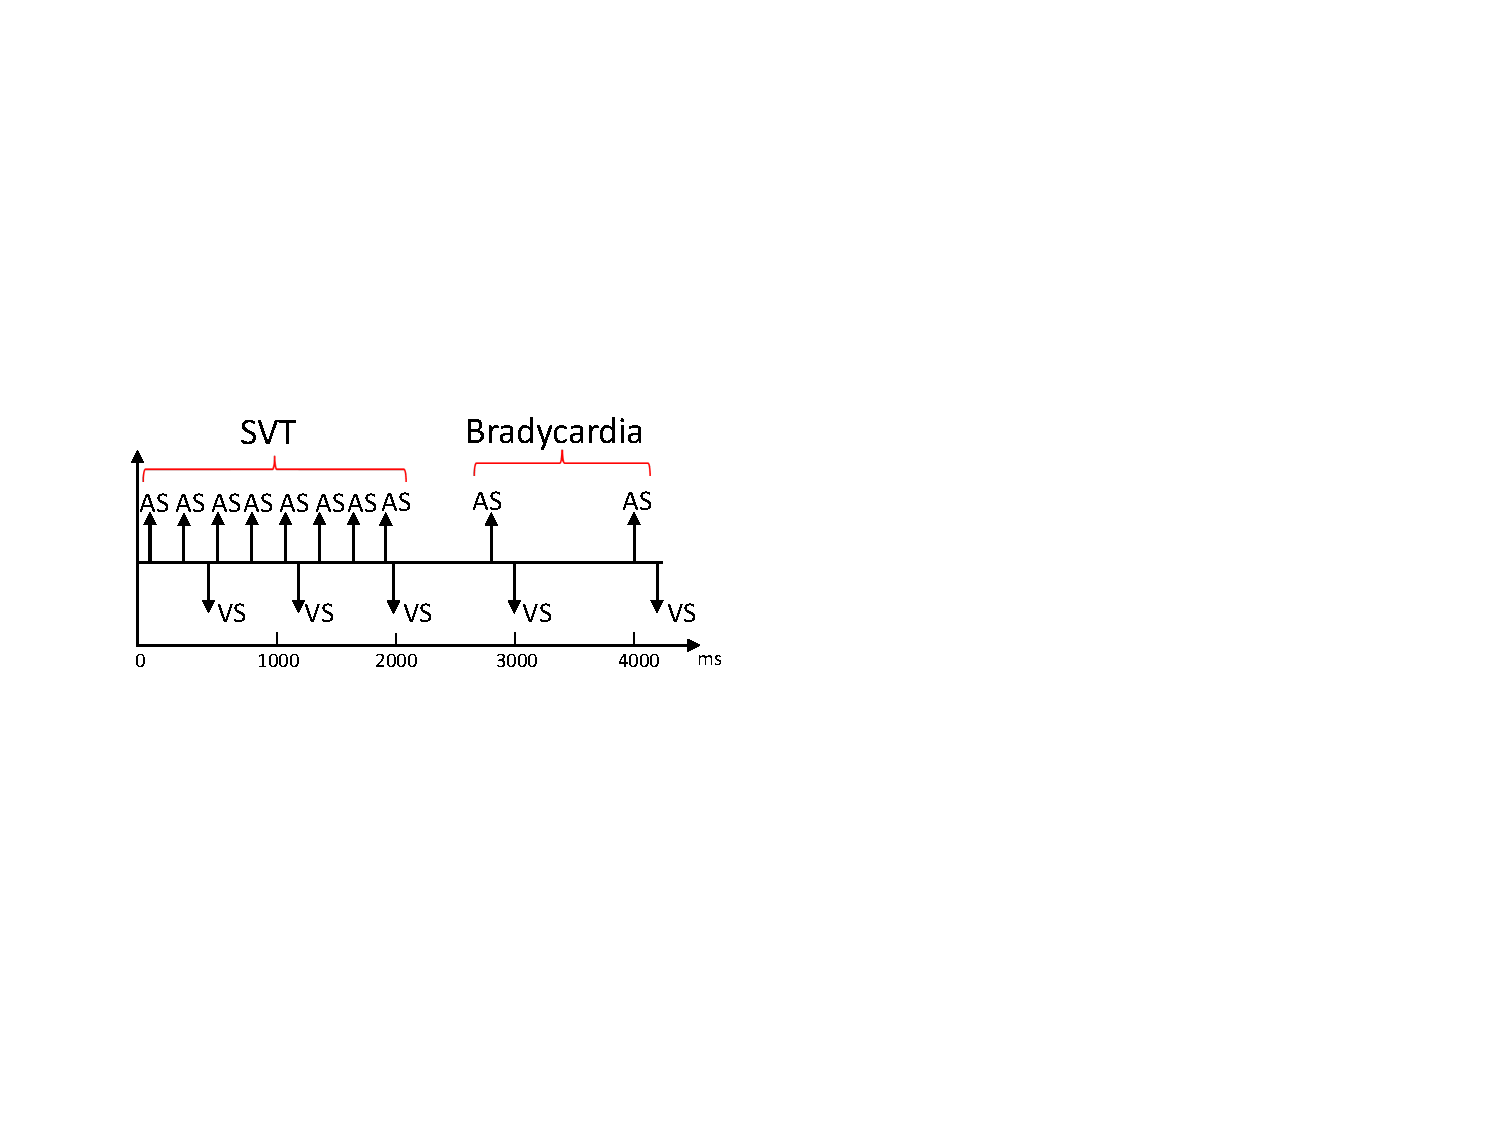
\includegraphics[width=0.4  \textwidth]{figs/SVT_none.pdf}
		\label{fig:SVT_none}
		} 
%	\hspace{.1in}%
		
		\subfigure [\small] 
		{
		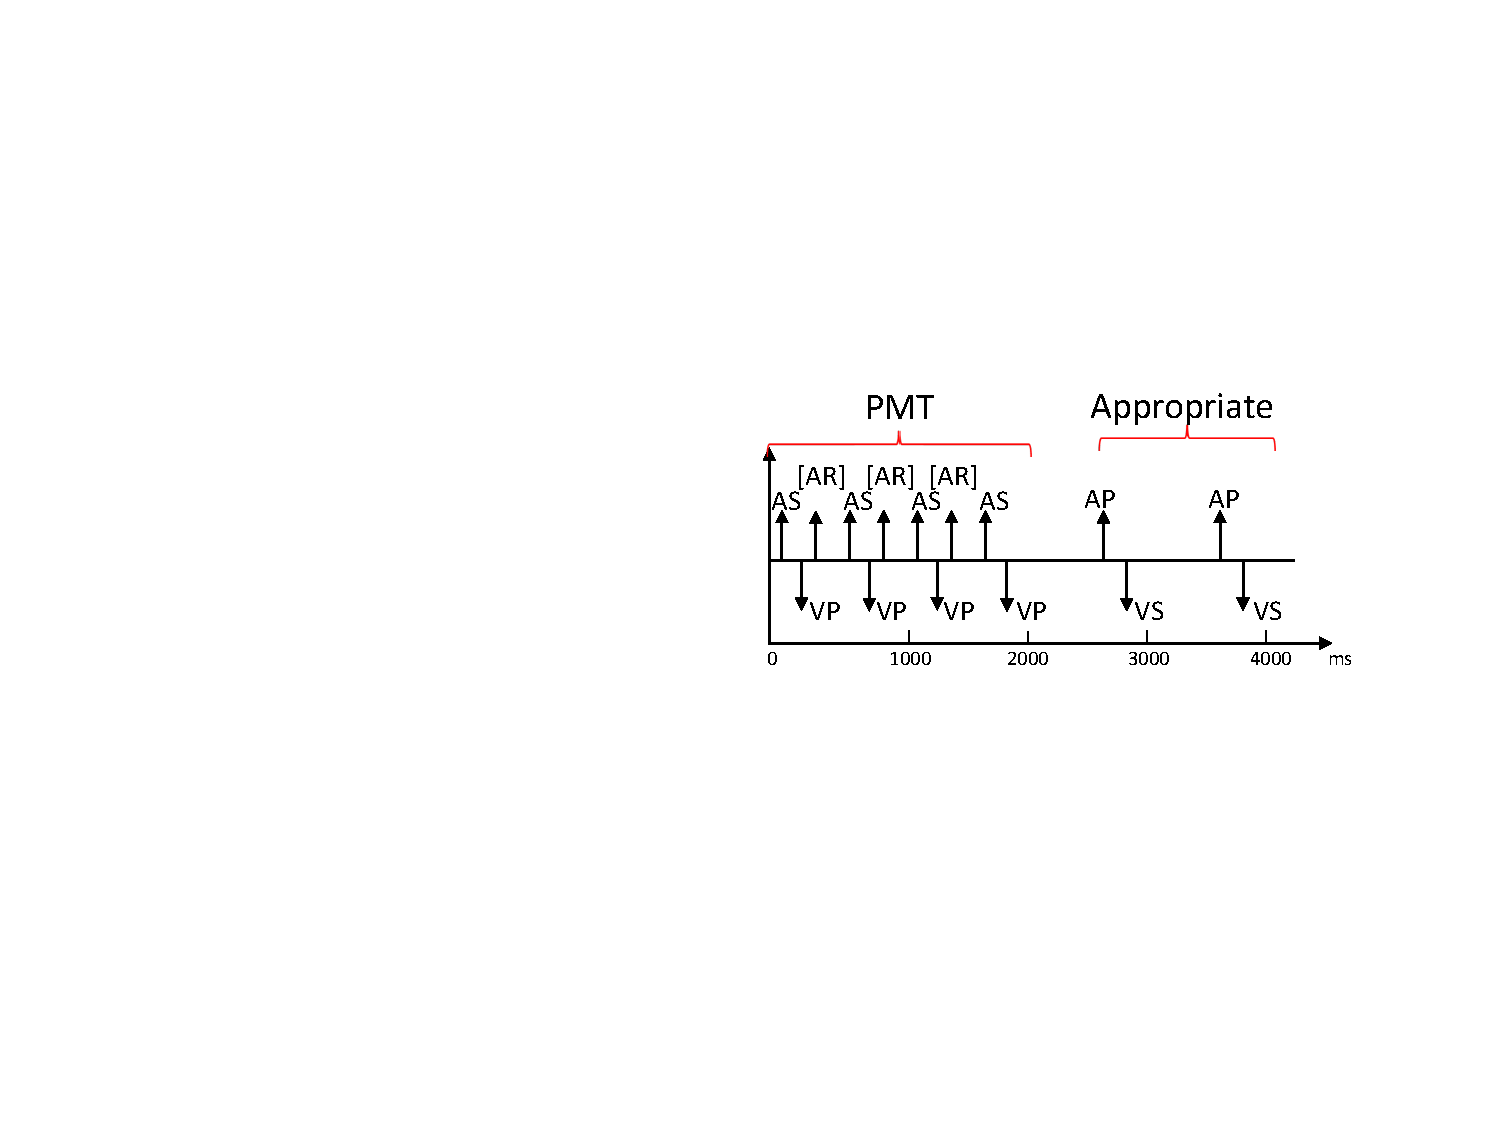
\includegraphics[width=0.4\textwidth]{figs/SVT_DDD.pdf}
		\label{fig:SVT_DDD}
		} 
%\vspace{-10pt}
\caption{\small (a) Node automaton. Dotted transition is only valid for pacemaker tissue like SA node; (b) Path automaton; (c) Model of the electrical conduction system of the heart using a network of node \& path automata~\cite{vhm_ecrts10}.}
%\vspace{-15pt}
\end{figure*} 

Pacemaker manufacturers have designed algorithm to detect and terminate this behaviors. Intuitively, the mode-switch algorithm first detects SVT. After confirmed detection, it switches the pacemaker from a dual-chamber mode to a single-chamber mode. During the single-chamber mode, the A-V synchrony function of the pacemaker is deactivated thus the ventricular rate is decoupled from the fast atrial rate. After the algorithm determines the end of SVT, it will switch the pacemaker back to the dual chamber mode. 

The mode-switch algorithm specification we use is similar to the one described in the Boston Scientific pacemakers manual \cite{compass}. The algorithm first measures the interval between atrial events outside the blanking period (AS, AR). The interval is considered as \emph{fast} if it is above a threshold (\emph{Trigger Rate}) and \emph{slow} otherwise. In our UPPAAL model we model it as $INT$ (see \figref{dur_count} (1)). A counter $CNT$ increments for \emph{fast} events and decrements for \emph{slow} events (see \figref{dur_count} (2)). After the counter value reaches the \emph{Entry Count}, the algorithm will start a \emph{Duration} ($DUR$) which is a time interval used to confirm the detection of SVT (see \figref{dur_count} (3)). In the \emph{Duration}, the counter keeps counting. If the counter value is still positive after the \emph{Duration}, the pacemaker will switch to the VDI mode (\emph{Fallback mode}). In the VDI mode, the pacemaker only senses and paces the ventricle. At any time if the counter reaches zero, the \emph{Duration} will terminate and the pacemaker is switched back to DDD mode.
% to show some interesting findings. The basic idea of this simplified model is explained in detail. \\
%\mySubSubSection{UPPAAL model for mode-switch algorithm}
In our UPPAAL model of the mode-switch algorithm, we use nominal parameter values from the clinical setting. We define \emph{trigger rate} at 170bpm (350ms), \emph{entry count} at 8, \emph{duration} for 8 ventricular events and \emph{fallback mode} as VDI. 

In order to model both DDD and VDI modes and the switching between them, we made modifications to the AVI and LRI components.
In each component two copies for both modes are modeled, and switch between each other when switching events (DDD, VDI) are received. During VDI mode, VP is delivered by the LRI component instead of the AVI component. The clock values are shared between both copies in order to preserve essential intervals even after switching. The modified AVI ($AVI'$) and LRI ($LRI'$)components are shown in \figref{avi_ms}. 
\begin{figure*}
		\centering
		%\vspace{-19pt}
		\includegraphics[width=0.8\textwidth]{figs/AVI_ms.pdf}
		%\vspace{-10pt}
		\caption{\small (a) After switching to \textsf{VDI} mode, the new LRI component \textsf{LRI'} maintains a minimum V-V interval; (b) After switching to \textsf{VDI} mode, the new AVI component \textsf{AVI'} keeps track of the time after each atrial events.}
		%  \vspace{-20pt}
		\label{fig:avi_ms}
\end{figure*}
\begin{figure*}
		\centering
				%\vspace{-15pt}
		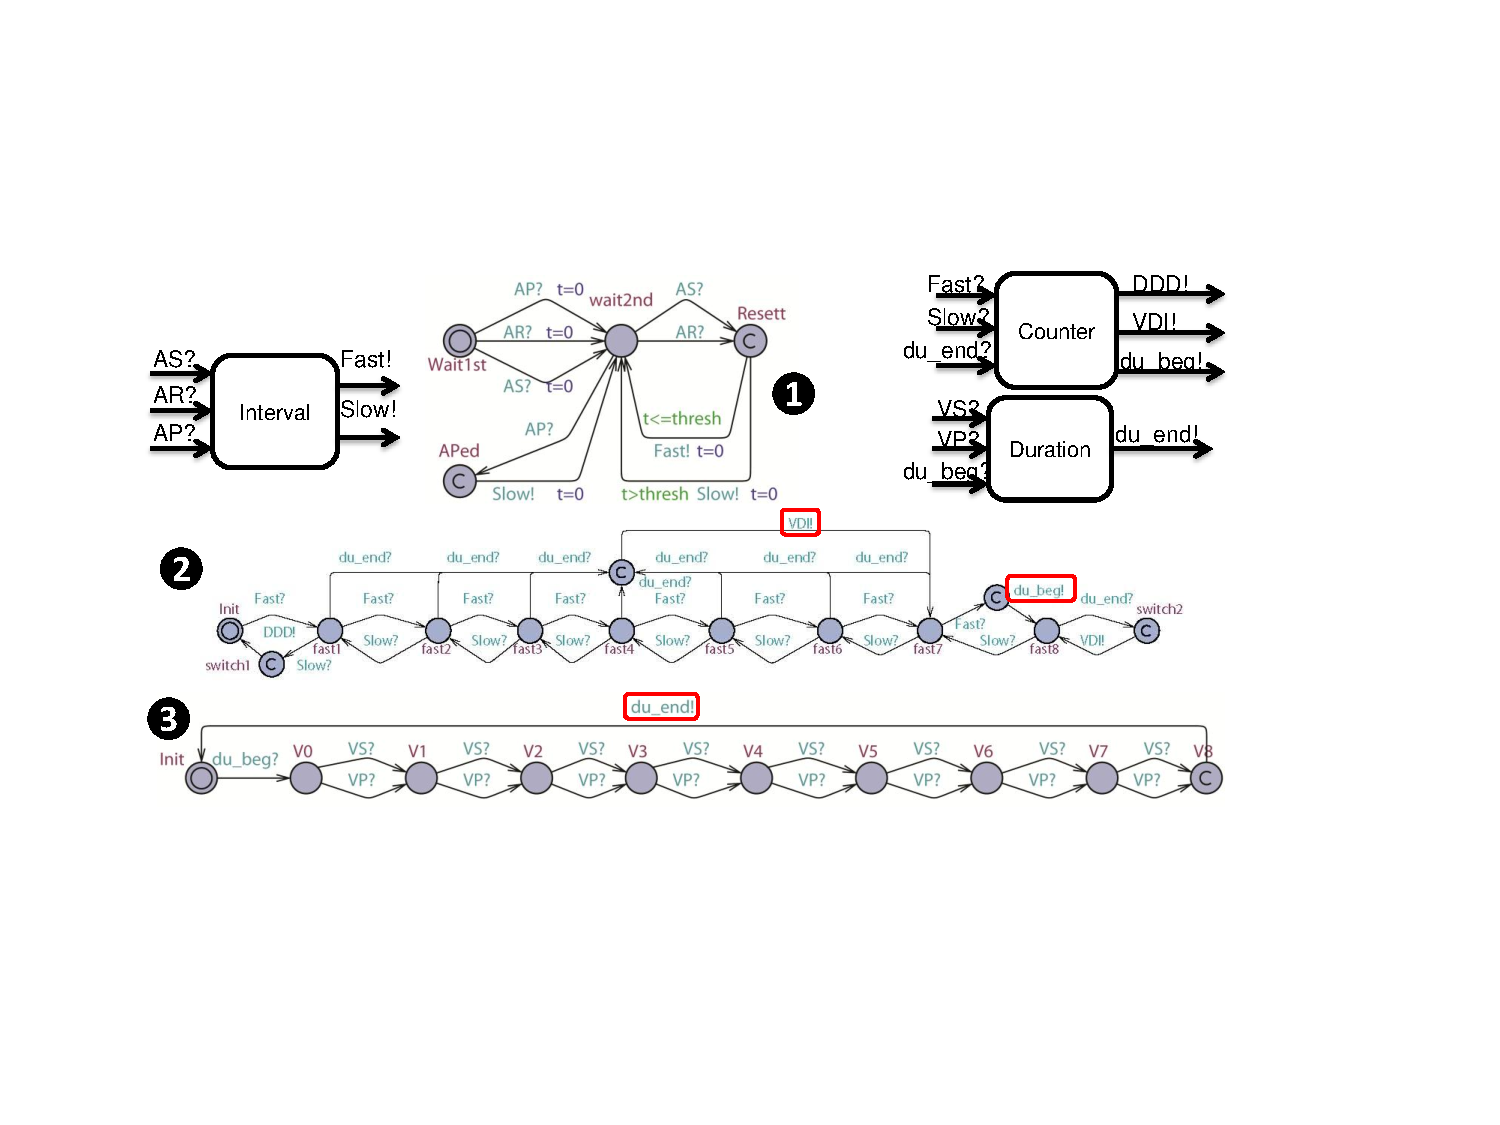
\includegraphics[width=0.9\textwidth]{figs/duration.pdf}
		\vspace{-10pt}
		\caption{\small (a) Component \textsf{INT} An atrial event (\textsf{AS,AR}) arrive before \textsf{thresh} after the previous atrial event is regarded as \textsf{fast} event. Atrial event arrive after \textsf{thresh} and \textsf{AP} are regarded as \textsf{slow} event; (b) Component \textsf{CNT} After 8 \textsf{fast} event the algorithm will start a duration by sending \textsf{du\_beg} and will switch to \textsf{VDI} mode when the duration ends (\textsf{du\_end}); (c) Component \textsf{DUR} The duration length is 8 ventricular events (\textsf{VS,VP})}
		  %\vspace{-15pt}
		\label{fig:dur_count}
\end{figure*} 

\chapter{Closed-loop Model Checking}
\begin{itemize}
	\item How to use models to cover environmental conditions specified in the physiological requirements, that the device may encounter?
            \item Can model checking find violations that testing cannot find?
            \item What are the effects of adding new features to the software? Can they disrupt the safety properties that the previous device hold?
            \item What is the model complexity requirements for each physiological requirement? When and how to refine the environment model?
            \item Exploring the whole state space sounds great. What are the limitations of model checking? 
\end{itemize}
In model-based software design, the system can be abstracted by a model. With proper model formalism and tools, the whole state space of the system can be checked
\begin{figure*}
\centering
%\vspace{-10pt}
		\subfigure[Monitor \textsf{PLRI\_test}] {
				\includegraphics[width=0.5\textwidth]{figs/LRI_test.pdf}
				\label{fig:safety1}
		} 
		\subfigure[Monitor \textsf{PURI\_test}] {	
			\includegraphics[width=0.45\textwidth]{figs/uri_test.pdf}
			\label{fig:uri_test}
		}
		%\vspace{-10pt}
	\caption{(a) Monitor for LRL: Interval between two ventricular events should be less than TLRI, (b) Monitor for URL: Interval between a ventricular event and a VP should be longer than TURI}
%\vspace{-15pt}
\end{figure*} 
\section{Reachability of Unsafe Regions}
The basic function of a pacemaker is to increase heart rate when necessary. As the result, we not only want to verify that the heart rate has been increased accordingly, but also ensure the pacemaker does not increase the heart rate too much. Since these requirements should hold for all possible heart conditions, the most abstract heart model $H_4$ is selected as the environment model. The following two requirements specify the unsafe regions  (too fast and too slow) within the closed-loop state space.

\subsection{Lower Rate Limit}
The most essential function for the pacemaker is to treat bradycardia by maintaining the ventricular rate above a certain threshold. We define the region where the ventricular rate is slow, as \textsf{unsafe}. The monitor \textsf{PLRI\_test} is designed to measure intervals between ventricular events and is shown in \figref{safety1}. For property \\
\textsf{$\varphi_{LRI}=$A[] (PLRI\_test.secV imply PLRI\_test.t$\leq$TLRI)}\\ we have $H_4\| P\| PLRI\_test\models\varphi_{LRI}$.

\subsection{Upper Rate Limit}
The pacemaker is not designed to treat tachycardia so it can only pace the heart to increase its rate and cannot slow it down. However, it is still important to guarantee it does not pace the ventricles beyond a maximum rate to ensure safe operations. To this effect, an Upper Rate Interval (URI) is specified such that the pacemaker can increase the ventricular rate up to this limit. 
  
We require that a ventricle pace (VP) can only occur at least $TURI$ after a ventricle event (VS, VP). The monitor \textsf{PURI\_test} is shown in \figref{uri_test}. For the property\\
$\varphi_{URI}=$\textsf{A[] (PURI\_test.secV imply PURI\_test.t$\geq$TURI)} \\
we have $H_4\| P\| PURI\_test\models \varphi_{URI}$.

\section{Model Checking the Mode-Switch Algorithm}

\subsection{Existence of PMT during SVT}
The monitor \textsf{Pv\_v} is designed to show existence of PMT during SVT. It goes to the error state if the ventricular rate drops below the Upper Rate Limit (\figref{vv}).  
\begin{figure}
		\centering
		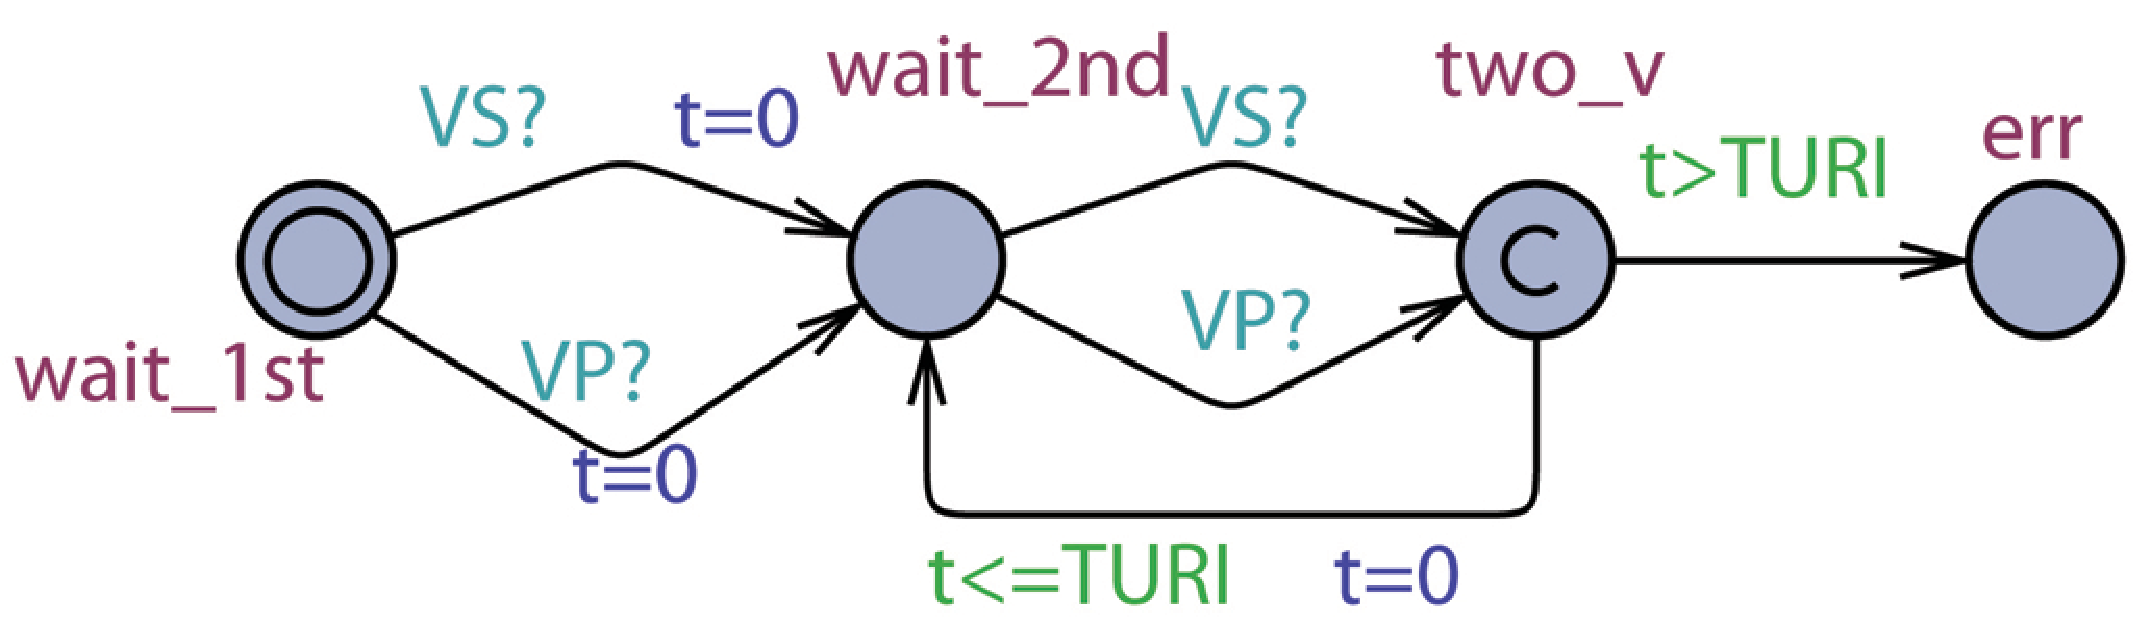
\includegraphics[width=0.4\textwidth]{figs/vv.pdf}
		\caption{\small Monitor \textsf{Pv\_v} for SVT: There exists an endless sequence in which interval between ventricular events is at most TURI}
		  %\vspace{-15pt}
		\label{fig:vv}
\end{figure}

We specify\\
$\varphi_{MS}=E[] (not Pv\_v.err)$\\
which verifies the existence of PMT. The heart model $H_3$ is not suitable for this property since the non-deterministic conduction of component $P_3$ does not capture the blocking property of the AV node, which is the key in PMT. We use a more refined model $H_2$ which has AV node modeled. To identify the PMT scenario, we first set $H_2.N^1.Trest\_min<100$ so that the atrial rate can be high and $H_2.N^2.Trest\_min>TURI$ so that the intrinsic heart rate is less than TURI. The property is first verified on pacemaker without the mode-switch algorithm. We have\\
$H_2\|P\|Pv\_v\models\varphi_{MS}$
and the evidence returned by the model checker illustrates the PMT scenario.

% There are two separate AVI and LRI components for each mode and switches to the corresponding ones when synchronization signals are received. The clock values are kept so that essential intervals are kept. 
\subsection{Verification against fundamental safety properties}
With the pacemaker with mode-switch algorithm: $P_2$=\textsf{LRI'$\|$AVI'$\|$URI$\|$PVARP$\|$VRP$\|$INT$\|$CNT$\|$DUR}, we verify the same fundamental safety properties on the pacemaker model with mode-switch algorithm. We have:
$$H_2\|P_2\|PURI\_test\models\varphi_{URI}$$
$$H_2\|P_2\|PLRI\_test\not\models\varphi_{LRI}$$
The Upper Rate Limit property still holds but the Lower Rate Limit property is violated. The counterexample is proved to be valid after checking the trace of more refined heart models. By analyzing the trace we found that when the pacemaker is switching from VDI mode to DDD mode, the responsibility to deliver VP switched from LRI component to AVI component. Since the clock reference is different (Ventricular events in LRI component and Atrial events in AVI component), the clock value for delivering the next VP is not preserved. As a result, if an atrial event which triggered the mode-switch from VDI to DDD happens within [TLRI-TAVI, TLRI) after the last ventricular event, the next ventricular pacing will be delayed by at most TAVI time, which violates the Lower Rate Limit property (\figref{safety}). 
\begin{figure}
		\centering
		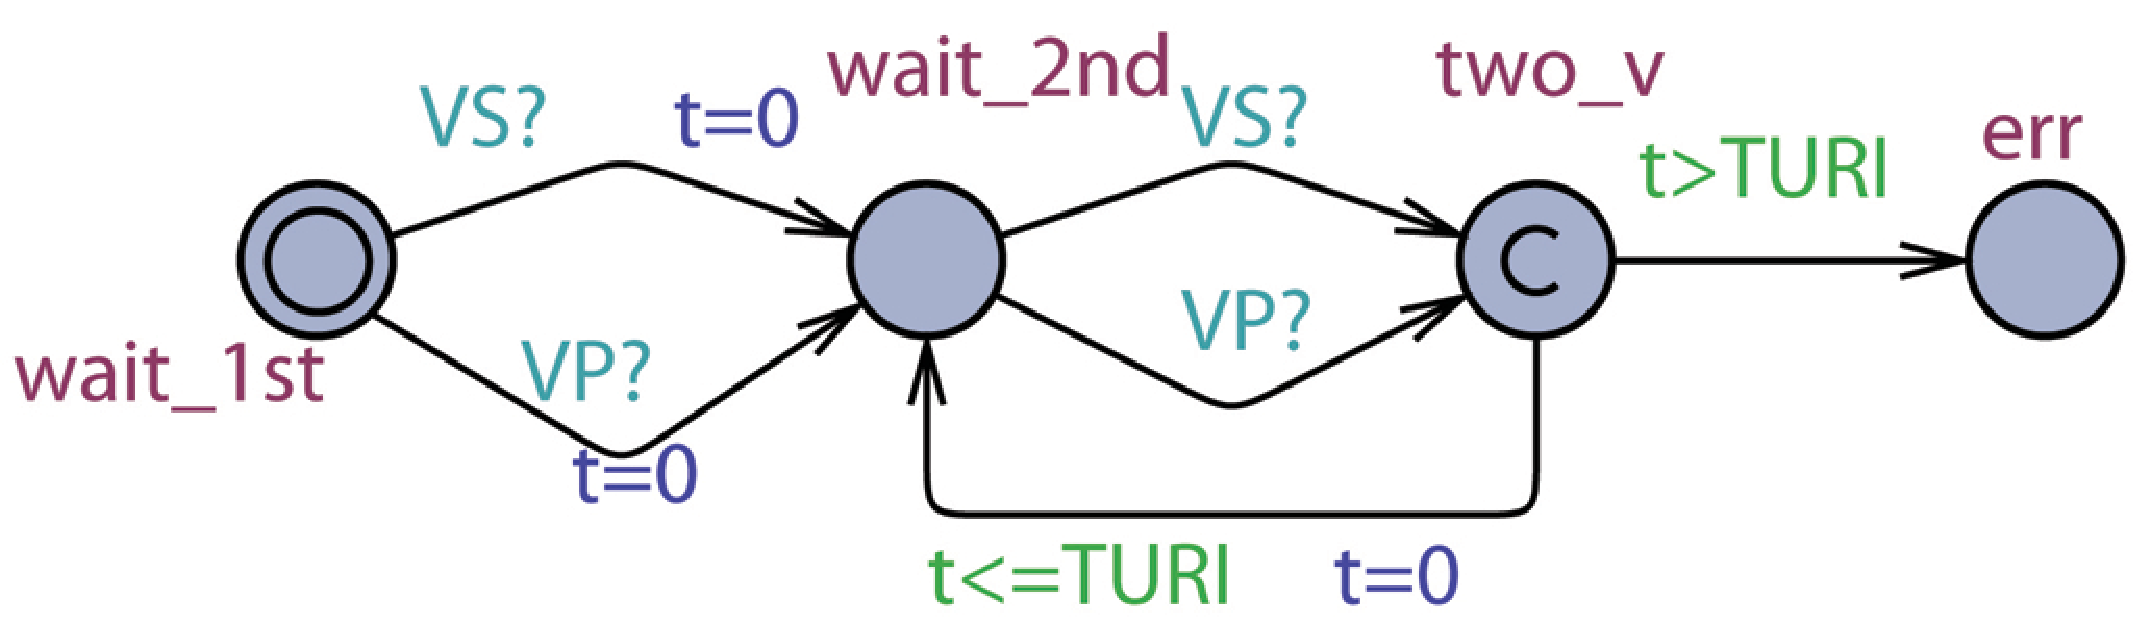
\includegraphics[width=0.4\textwidth]{figs/vv.pdf}
		\caption{\small Monitor \textsf{Pv\_v} for SVT: There exists an endless sequence in which interval between ventricular events is at most TURI}
		  %\vspace{-15pt}
		\label{fig:vv}
\end{figure}
\subsection{Verification of the Mode-switch Algorithm}
After implementing the Mode-switch algorithm, we verified the model against the same existence property. We expect the violation of this property, since during VDI mode the ventricular rate of the heart model is less than the Upper Rate Limit and will not trigger ventricular pacing. However, this property is still satisfied, indicating the mode-switch algorithm failed to eliminate the PMT scenario. The evidence trace returned by UPPAAL shows that a subset of atrial events fall into the blanking period after a ventricular event (see \figref{liveness}). As a result, two fast events are reduced to one slow event and mode switch may never happen. This scenario does exist in all our refined heart models, we conclude that the trace is physiologically feasible. The mode-switch algorithm in our pacemaker model can not terminate all PMT behaviors as specified.
\begin{figure}
\centering
%\vspace{-20pt}
		\subfigure []{
				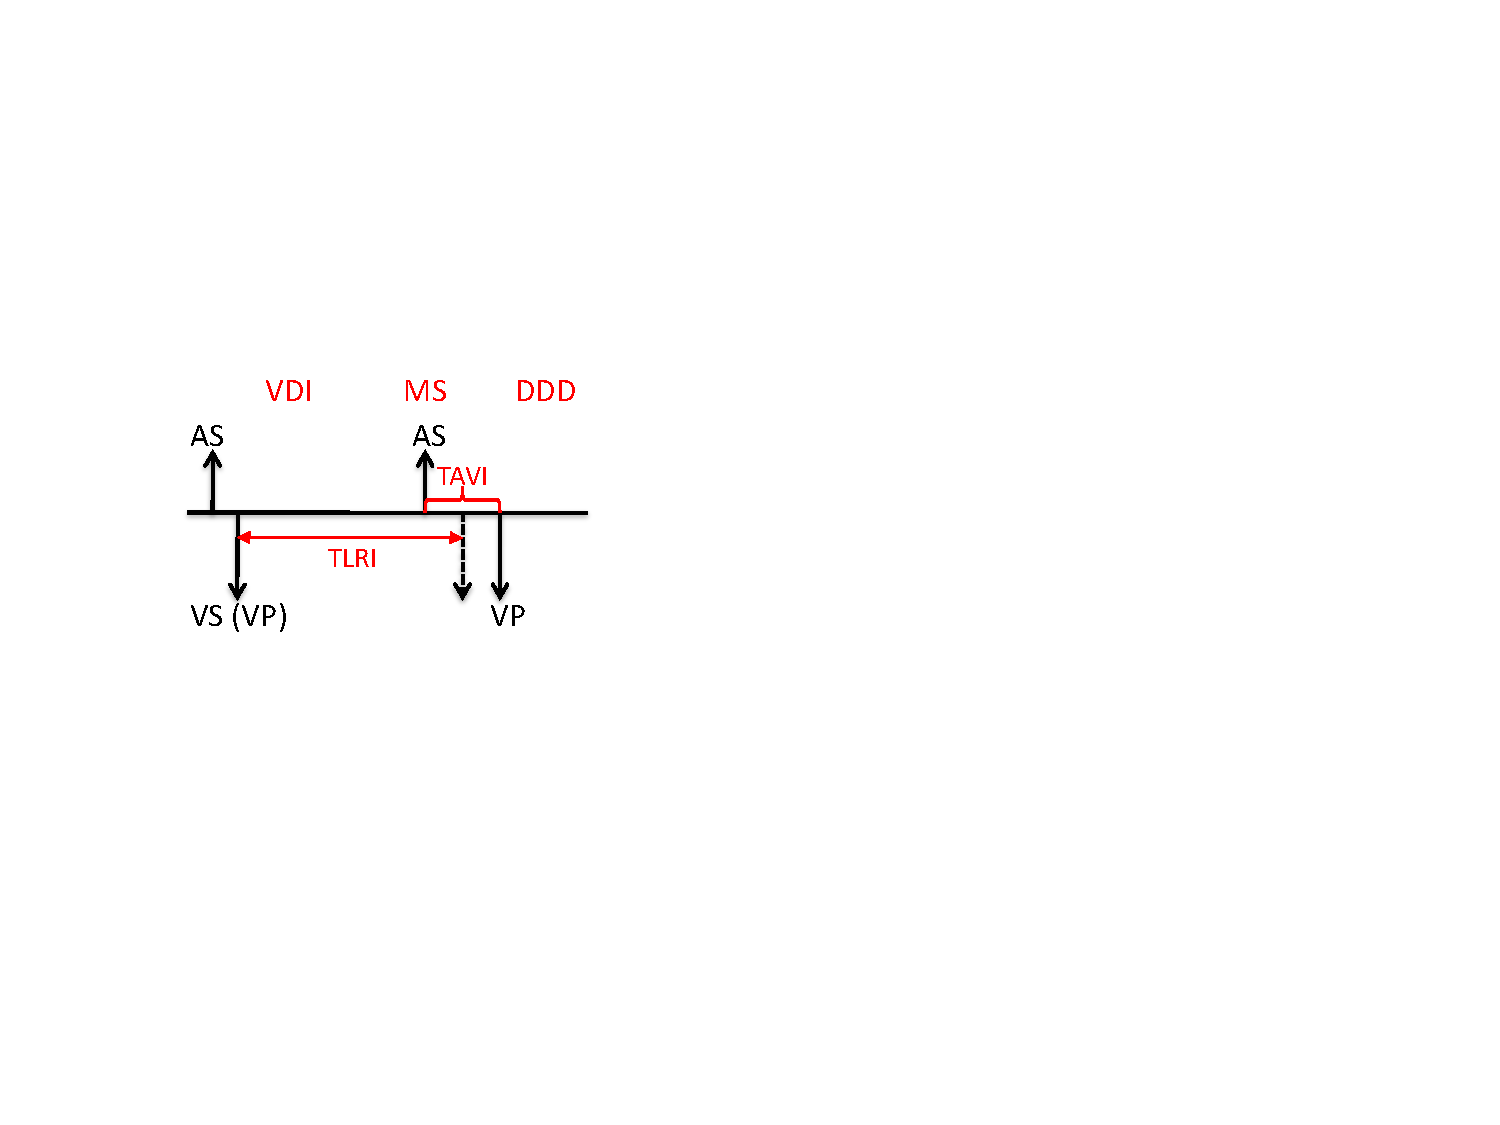
\includegraphics[width=0.4\textwidth]{figs/safety.pdf}
				\label{fig:safety}
		} 
		\subfigure []{	
			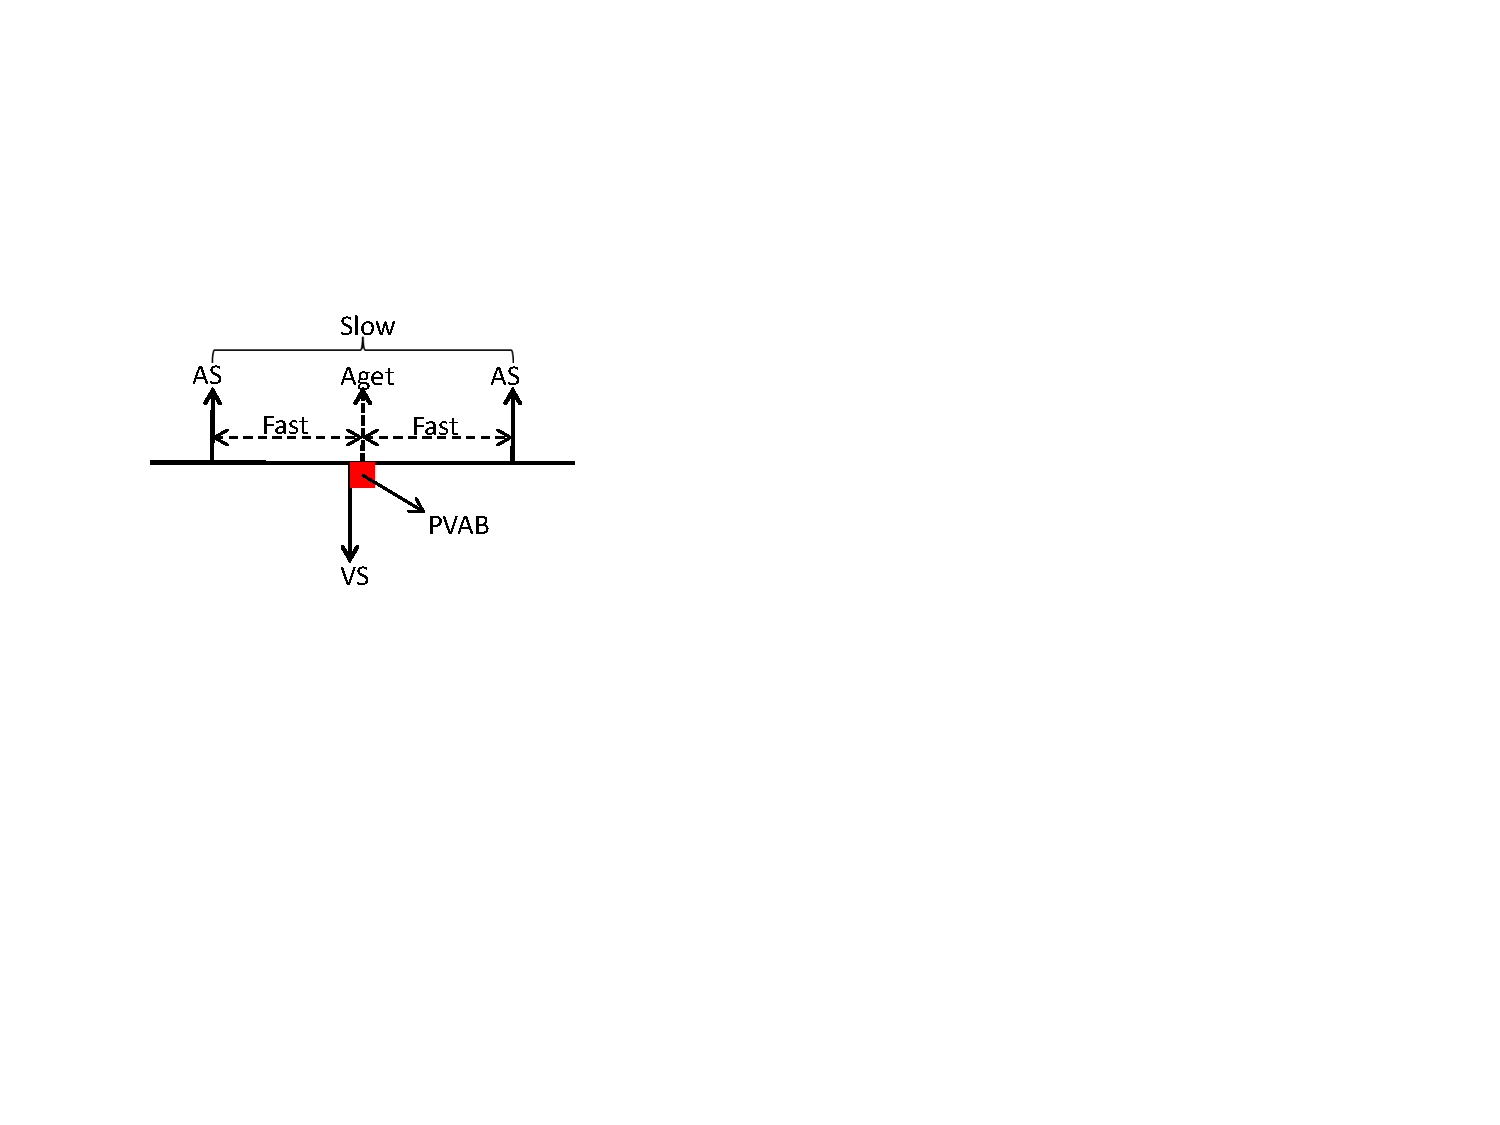
\includegraphics[width=0.4\textwidth]{figs/liveness.pdf}
			\label{fig:liveness}
		}
		\vspace{-10pt}
	\caption{(a) Safety Violation: VP is delayed due to the reset of timer during mode-switch, (b) Correctness Violation: The blocking period may block some atrial events, turning two \emph{Fast} events to one \emph{Slow} event \cite{TACAS12}}
\vspace{-20pt}
\end{figure} 
\section{Abstraction Tree for Environment Modeling}

\subsection*{Step 1: Abstraction Tree Construction}
A set of heart models corresponding to different heart conditions are first developed. 
The list can be expanded as new heart conditions are discovered.
Because we start from a set of initial models, and each one may be abstracted using a number of abstraction rules, we have a choice of which rules to apply to which models, and the order in which to apply them. More details of the abstraction rules can be found in \cite{REGAR_tech}
Depending on which rule is applied when, we end up with different abstract models.
Thus an \emph{abstraction tree} $T_{HM}$ for the heart is created, as shown in \figref{HM_abs}. 
%Note that applying rules in different order results different abstraction tree. 
%The order used to obtain $HM\_tree$ is based on the domain knowledge that certain heart conditions may have similar behaviors and similar inputs to the pacemaker. 
%This systematic grouping maintains the physiological-relevance of the heart model even at higher abstraction levels, and reduce the necessity to resolve ambiguities at lower abstraction levels when model checking certain requirements.
\begin{figure}[!t]
	\centering
	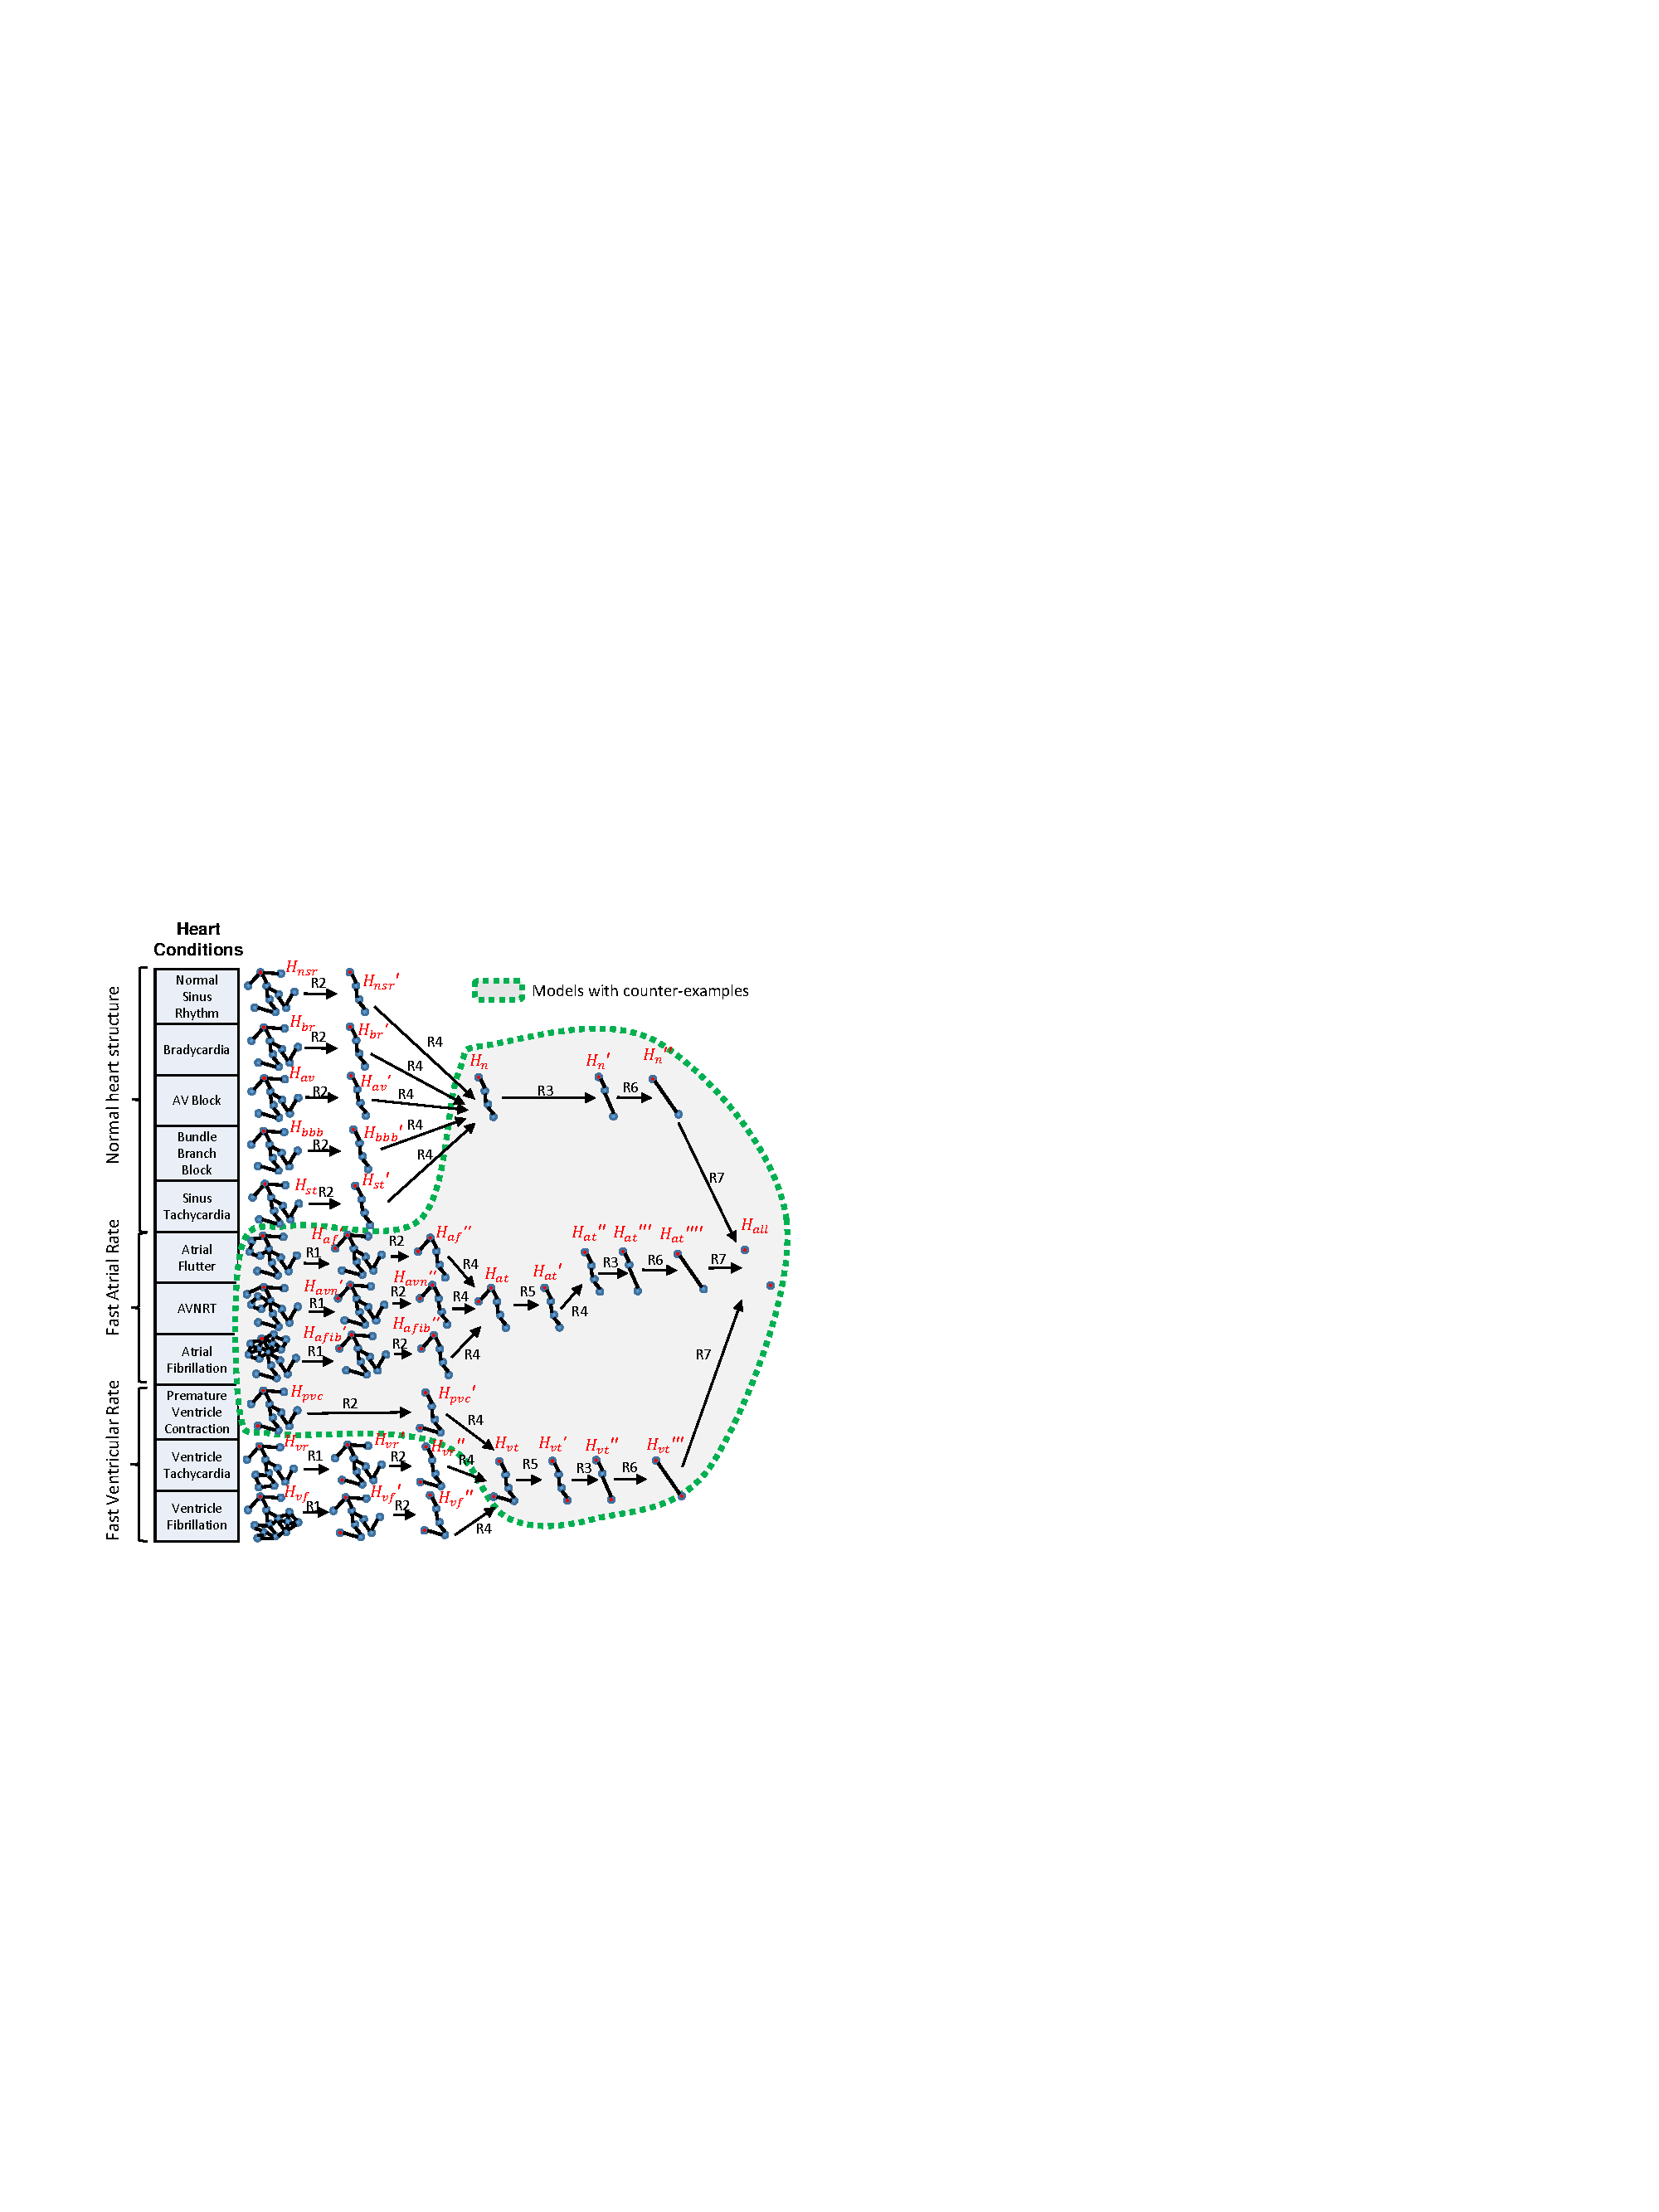
\includegraphics[width=0.85\textwidth]{figs/abs.pdf}
	%\vspace{-5pt}
	\caption{\small Heart Model Abstraction Tree}
	\vspace{-15pt}
	\label{fig:HM_abs}
\end{figure}

\subsection*{Step 2: Requirement Encoding}
The following requirement is designed to prevent the pacemaker from pacing too fast: 
``If the intervals between self-activations of the atria are between 300ms to 1000ms (60bpm-200bpm), the intervals between ventricular paces should be no shorter than 500ms.''
Self-activation of the atria can be expressed using the location and clock of of node automaton $N_A$.
The requirement can be formalized using the monitor  $M_{sing}(VP,500,\infty)$:
%\hatodo{mention $N_A$ is the atrium node automaton}
\[Req1: N_A.loc=Rest \land N_A.t\in [300,1000] \Rightarrow \neg M_{sing}.loc==Err\]
%\todo[inline]{some figure captions are all caps, others are not. please use same thing throughout}
%\begin{figure}[!b]
	%\centering
	%\vspace{-10pt}
	%\includegraphics[width=0.5\textwidth]{figs/abs_sim.pdf}
%
	%\caption{\small Abstraction Rule Application Example}
%\vspace{-10pt}
	%\label{fig:abs_exam}
%\end{figure}
 \subsection*{Step 3: Choosing Appropriate Heart Models For the Requirement}
To verify the closed-loop system with pacemaker model $PM$ and abstraction tree $T_{HM}$ (\figref{HM_abs}) against requirement $Req1$, the most abstract appropriate models are selected from the tree. 
The single event monitor $M_{sing}$ from \figref{monitor}.a with variables $Var(M_{sing})=\{M_{sing}.t,M_{sing}.loc\}$ is used for this requirement. 
The variables in the requirement are:
$Var(Req1)=\{N_A.t,N_A.loc,M_{sing}.loc\}$.

At the root of the tree $H_{all}$, we have $\{N_A.t,N_A.loc\} \not \subset Var(H_{all})\cup Var(M_{sing})$. 
So $H_{all}$ is not appropriate for $Req1$. 
All the children of $H_{all}$: $H_n'',H_{at}'''',H_{vt}'''$ are appropriate for $Req1$,
%we have $Var(Req1)\cup Var(M_{sing})\subset Var(H_n'')=Var(H_{at}'''')=Var(H_{vt}''')$, 
thus these 3 heart models are output as the most abstract models that are appropriate for $Req1$.
\begin{figure}[!t]
	\centering
	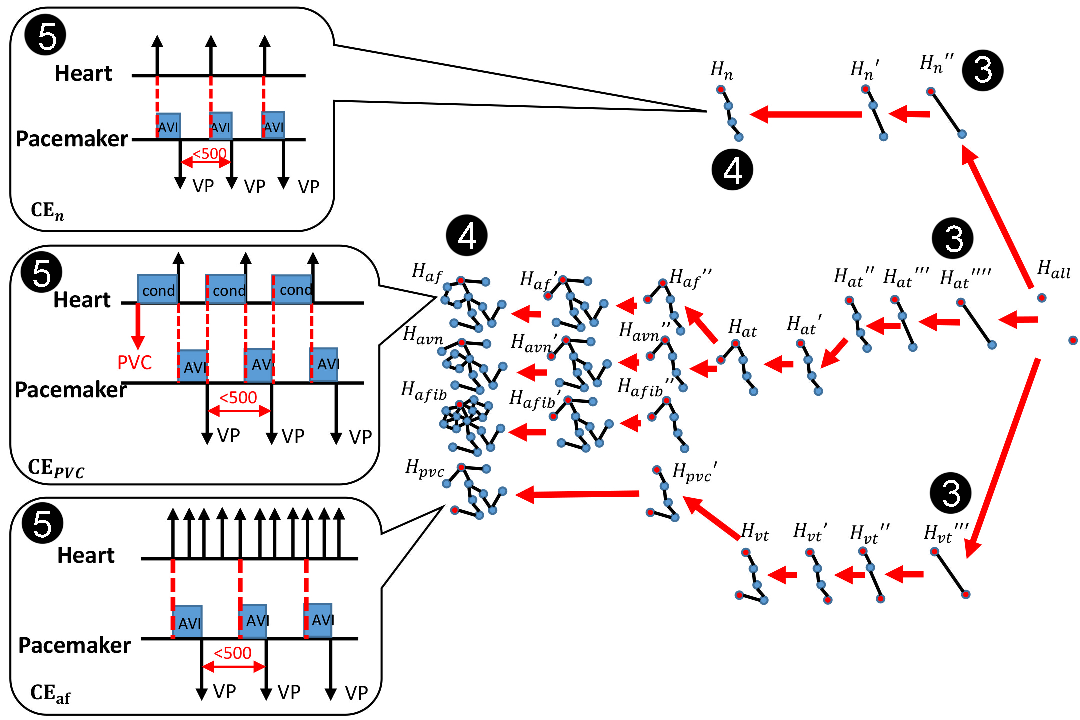
\includegraphics[width=0.8\textwidth]{figs/abs_rev.pdf}
	%\vspace{-5pt}
	\caption{\small Finding the most concrete counter-examples using the abstraction tree}
	\vspace{-10pt}
	\label{fig:CE}
\end{figure}
	\vspace{-10pt}
\subsection*{Step 4: Return the most Concrete Counter-Examples}
After the appropriate models for $Req1$ are selected, we have the initial set
$HM=\{H_n'',H_{at}'''',H_{vt}'''\}$.
Then we run Algorithm 2. By model checking on all 3 initial models in UPPAAL we have: 
$$H_n''||PM\not\models Req1;\; H_{at}''''||PM\not\models Req1;\; H_{vt}'''||PM\not\models Req1$$
%$$[1,[]]=ModelChecking(H_n'',PM,Req1)$$
 %$$[0,CE_1]=ModelChecking(H_{at}'''',PM,Req1)$$
%$$[0,CE_2]=ModelChecking(H_{vt}''',PM,Req1)$$
%\hatodoin{In the following text you use $CE_{at}$, etc. It's  best to use the letter subscripts in the above equations as well, so it's clear which cex comes from which heart model.}
%For the two heart models $H_{at}'''',H_{vt}'''$ in which the requirement is violated, the algorithm keeps going down the abstraction tree, and upon termination counter-examples are returned for the following heart models
The abstraction tree is then further explored. The heart models with counter-examples are illustrated in \figref{HM_abs}, and the most refined heart models with counter-examples are: $H_{n};H_{pvc};H_{af};H_{avn};H_{afib}$.
%$$[0,CE_{at}]=ModelChecking(H_{at},PM,Req1)$$
%$$[0,CE_{pvc}]=ModelChecking(H_{pvc},PM,Req1)$$
%$$[0,CE_{af}]=ModelChecking(H_{af},PM,Req1)$$
%$$[0,CE_{avn}]=ModelChecking(H_{avn},PM,Req1)$$
%$$[0,CE_{afib}]=ModelChecking(H_{afib},PM,Req1)$$

%\begin{figure}[!t]
		%\centering
		%\includegraphics[width=0.9\textwidth]{figs/case.pdf}
		%%\vspace{-5pt}
		%\caption{\small Counter-examples}
		  %\vspace{-10pt}
		%\label{fig:CE}
%\end{figure}
	\vspace{-10pt}
\subsection*{Step 5: Analysis of the Counter-examples}
The counter-examples are then shared with physicians for analysis. In \figref{CE} we demonstrate 3 counter-examples. In the counter-examples, the first signal shows the intrinsic heart signals over time with up arrows as atrial activations and down arrows as ventricular activations. The second signal shows the pacemaker outputs with up arrows as atrial pacing and down arrows as ventricular pacing.%We only show the activations of the atrial node and ventricle pacing. 

$CE_{n}$ is returned by $H_n$ and none of its children models violate the requirement. By careful analysis we found that $CE_{n}$ features the combination of fast intrinsic atrial rate and prolonged A-V conduction delay, which is the combination of heart conditions $H_{st}$ and $H_{av}$. This scenario shows that the abstraction rules can introduce physiological heart conditions that were not explicitly modeled in the initial model set. The pacemaker improved the open-loop heart condition by pacing the ventricles $AVI$ after each atrial event, which is a correct operation of the pacemaker despite the requirement violation. %\hatodo{is it TAVI or AVI like in the previous seciton?}

%\hatodoin{Do you mean that $CE_{at}$ is not a bug? Does this mean that the requirement may be violated in ways that are not dangerous?}
$CE_{pvc}$ has a very similar execution to $CE_{n}$. However, the activations of the atrial node are triggered by retrograde conduction from ventricular paces (marker \textsf{cond}). The atrial activations trigger another ventricular pace after $AVI$, which will trigger another retrograde conduction. In this case the heart rate is inappropriately high, which corresponds to a dangerous closed-loop behavior referred to as \emph{Endless Loop Tachycardia}.

In $CE_{af}$ the atrial rate is very high, which is also a sub-optimal but not dangerous heart condition. 
However, the ventricular rate can stay normal due to the blocking property of the AV node. 
Despite the filters in the pacemaker, the pacemaker still paces the ventricle for every 3 atrial activations, which extends fast atrial rate to more dangerous fast ventricular rate. 
%\hatodoin{Not very clear..do you mean that the intrinsoc centricular rate is fine because of AV filtering, but the PM is accelarating it?}
This scenario is referred to as Atrial Tachycardia Response of a pacemaker. 

From the analysis, pacemaker operations in $CE_{pvc}$ and $CE_{af}$ must be revised. However, the revision should not affect the behavior in $CE_{n}$. This example demonstrates that counter-examples from refined models provide more physiological context of the requirement violations, and distinguish the physiological conditions that can trigger the violations. The information is helpful for debugging and improving the algorithm. The physicians can also improve the physiological requirement so that these heart conditions can be then considered case by case.
